\documentclass{beamer}

\usepackage{Archivo}
\renewcommand{\sfdefault}{\rmdefault}
\usepackage{graphicx}
\usepackage{tikz}
\usetikzlibrary{calc}
\usepackage[most]{tcolorbox}

%% ---- Superteam Poland brand colors ----
\definecolor{stpldark}{HTML}{0B0E0F}   % near-black background
\definecolor{stplcard}{HTML}{161A1B}   % card / block surface
\definecolor{stplborder}{HTML}{1E2526}  % subtle track color for progress bar
\definecolor{stplred}{HTML}{DC143C}    % brand crimson red
\definecolor{stplwhite}{HTML}{FFFFFF}  % white
\definecolor{stplmuted}{HTML}{8A9BA8}  % muted / secondary text

\usetheme{default}
\setbeamersize{text margin left=0.85cm, text margin right=0.85cm}

%% ---- Background & base text ----
\setbeamercolor{background canvas}{bg=stpldark}
\setbeamercolor{normal text}{fg=stplwhite, bg=stpldark}
\usebeamercolor{normal text}

%% ---- Background image helpers ----
\newcommand{\stpldefaultbg}{%
  \setbeamertemplate{background}{%
    \begin{tikzpicture}[remember picture, overlay]
      \node[at=(current page.center), inner sep=0pt] {%
        
\includegraphics[width=\paperwidth,height=\paperheight]{images/bg-default.png}%
      };
      \fill[stplborder]
        (current page.north west) rectangle
        ([yshift=-2.5pt]current page.north east);
      \pgfmathsetmacro{\stplprog}{\insertframenumber/\inserttotalframenumber}
      \fill[stplred]
        (current page.north west) rectangle
        ($(current page.north west)+(\stplprog\paperwidth,-2.5pt)$);
    \end{tikzpicture}%
  }%
}
\newcommand{\stplherobg}{%
  \setbeamertemplate{background}{%
    
\includegraphics[width=\paperwidth,height=\paperheight]{images/bg-hero.png}%
  }%
}
\stpldefaultbg

%% ---- Structure ----
\setbeamercolor{structure}{fg=stplred}

%% ---- Title slide metadata ----
\setbeamercolor{title}{fg=stplwhite}
\setbeamercolor{subtitle}{fg=stplred}
\setbeamercolor{author}{fg=stplwhite}
\setbeamercolor{institute}{fg=stplmuted}
\setbeamercolor{date}{fg=stplmuted}

%% ---- Frame title: flat, no box background ----
\setbeamercolor{frametitle}{fg=stplwhite, bg=}
\setbeamerfont{frametitle}{size=\large, series=\bfseries}
\setbeamertemplate{frametitle}{%
  \vspace{0.35cm}%
  {\centering\insertframetitle\par}%
  \nointerlineskip\vspace{0.18cm}%
  \hfil{\color{stplred}\rule{2.2cm}{1.5pt}}\hfil\par%
}



%% ---- Incremental reveals ----
\beamerdefaultoverlayspecification{<+->}

%% ---- Bullet items ----
\setbeamercolor{itemize item}{fg=stplred}
\setbeamercolor{itemize subitem}{fg=stplmuted}
\setbeamercolor{itemize subsubitem}{fg=stplmuted}
\setbeamertemplate{itemize item}{\bfseries\textendash}
\setbeamertemplate{itemize subitem}{\small\textendash}
\setbeamercolor{enumerate item}{fg=stplred}
\setbeamercolor{enumerate subitem}{fg=stplmuted}

%% ---- Blocks (flat left-accent via tcolorbox) ----
\tcbset{
  stplbase/.style={
    enhanced, breakable,
    colback=stplcard, coltext=stplwhite,
    coltitle=stplwhite, fonttitle=\bfseries,
    boxrule=0pt, leftrule=3pt,
    arc=0pt, outer arc=0pt,
    top=5pt, bottom=5pt, left=7pt, right=7pt,
    toptitle=4pt, bottomtitle=4pt,
    titlerule=0pt,
  },
}
\renewenvironment{block}[1]{%
  \begin{tcolorbox}[stplbase, colframe=stplred, title={#1}]%
}{%
  \end{tcolorbox}%
}
\renewenvironment{alertblock}[1]{%
  \begin{tcolorbox}[stplbase, colframe=stplred!75!black,
    colback=stplred!10!stplcard, title={#1}]%
}{%
  \end{tcolorbox}%
}
\renewenvironment{exampleblock}[1]{%
  \begin{tcolorbox}[stplbase, colframe=stplmuted, title={#1}]%
}{%
  \end{tcolorbox}%
}

%% ---- Table of contents ----
\setbeamercolor{section in toc}{fg=stplwhite}
\setbeamercolor{subsection in toc}{fg=stplmuted}
\setbeamertemplate{section in toc}{%
  {\color{stplred}\textbf{\textendash}}\hspace{0.5em}\inserttocsection%
}

%% ---- Footline: minimal ----
\setbeamertemplate{footline}{%
  \begin{beamercolorbox}[wd=\paperwidth, ht=0pt, dp=0.55cm]{normal text}%
    \hspace{0.85cm}%
    
\includegraphics[height=1.6ex]{images/stpl-logo.png}%
    \hfill%
    \textcolor{stplmuted}{\tiny\insertframenumber\,/\,\inserttotalframenumber}%
    \hspace{0.85cm}%
  \end{beamercolorbox}%
}
\setbeamertemplate{navigation symbols}{}

%% ---- Title frame helper (uses hero background) ----
\newcommand{\maketitleframe}{%
  \stplherobg
  \begin{frame}[plain]%
    \titlepage%
  \end{frame}%
  \stpldefaultbg
}

%% ---- Section divider slides ----
\AtBeginSection[]{%
  \stplherobg
  \begin{frame}[plain]
    \begin{tikzpicture}[remember picture, overlay]
      \fill[stplred, opacity=0.07]
        ([xshift=-2.5cm]current page.east) circle (5.5cm);
      \fill[stplred]
        (current page.north west) rectangle ([xshift=5pt]current page.south west);
    \end{tikzpicture}%
    \vfill
    \hspace{0.1\paperwidth}%
    \begin{minipage}{0.8\paperwidth}
      \textcolor{stplmuted}{\small Section \thesection}\\[0.35cm]
      {\color{stplwhite}\LARGE\bfseries\insertsectionhead}\\[0.25cm]
      {\color{stplred}\rule{3cm}{1.5pt}}
    \end{minipage}%
    \vfill
  \end{frame}%
  \stpldefaultbg
}

%% ---- Title page ----
\setbeamertemplate{title page}{%
  \begin{tikzpicture}[remember picture, overlay]
    \fill[stplred]
      (current page.north west) rectangle ([xshift=5pt]current page.south west);
    \fill[stplred, opacity=0.07]
      ([xshift=-3cm,yshift=3cm]current page.north east) circle (5.5cm);
    \fill[stplred, opacity=0.04]
      ([yshift=-1.5cm]current page.south east) circle (3.5cm);
  \end{tikzpicture}%
  \vfill
  \hspace{0.08\paperwidth}%
  \begin{minipage}{0.85\paperwidth}
    
\includegraphics[width=3cm]{images/stpl-logo.png}\par
    \vspace{0.8cm}
    {\usebeamerfont{title}\usebeamercolor[fg]{title}\inserttitle}\par
    \vspace{0.2cm}
    {\color{stplred}\rule{3cm}{1.5pt}}\par
    \vspace{0.3cm}
    {\usebeamerfont{subtitle}\usebeamercolor[fg]{subtitle}\insertsubtitle}\par
    \vspace{0.65cm}
    {\usebeamerfont{author}\usebeamercolor[fg]{author}\insertauthor}\par
    \vspace{0.12cm}
    {\small\textcolor{stplmuted}{\insertinstitute\enspace·\enspace\insertdate}}
  \end{minipage}%
  \vfill
}


\usepackage[utf8]{inputenc}
\usepackage[T1]{fontenc}
\usepackage{amsmath}

\title{Lending na Solanie}
\subtitle{Pożyczki bez banku --- Solana Bootcamp}
\author{}
\institute{Superteam Poland}

\begin{document}

\maketitleframe

\begin{frame}{Plan}
  \tableofcontents
\end{frame}

% ================================================================
\section{Drugi filar DeFi}

\begin{frame}{Drugi filar}
  \begin{itemize}
    \item Poprzednia lekcja zamknęła wymianę tokenów --- bez giełdy, bez animatora rynku
    \item Drugi filar obietnicy z Lekcji 0 --- \textbf{pożyczki bez banku}
    \item Bank ocenia zdolność, prowadzi rejestr, ściąga dług --- co go zastąpi w kodzie?
    \item Cała mechanika musi się zamknąć w smart kontrakcie i puli tokenów
  \end{itemize}
  \vspace{0.25cm}
  \begin{alertblock}{Bez oceny kredytowej}
    Łańcuch nie wie, kim jest pożyczkobiorca. Skoro nie ma scoringu ---
    co broni protokół przed niespłaconym długiem?
  \end{alertblock}
\end{frame}

\begin{frame}{Jak to działa}
  \begin{center}
    \begin{tikzpicture}[
        every node/.style={font=\scriptsize\bfseries},
        box/.style={
          draw=stplred, line width=1pt,
          fill=stplcard, text=stplwhite,
          rounded corners=2pt,
          minimum width=1.4cm, minimum height=0.55cm,
          align=center,
        },
        arr/.style={-latex, draw=stplred, line width=1pt},
        lbl/.style={font=\tiny\itshape, text=stplmuted},
      ]
      % Stage 1: Lender and Pool
      \node[box] (lender) {Lender};

      \node[draw=stplred, line width=1pt, fill=stplcard,
            rounded corners=2pt,
            minimum width=2.4cm, minimum height=0.85cm,
            right=1.8cm of lender] (pool) {};
      \node[font=\tiny\itshape, text=stplmuted]
            at ($(pool.north)+(0,5pt)$) {Pula};
      \node[font=\tiny\bfseries, text=stplred]
            at ($(pool.center)+(-0.55cm,0.08cm)$) {USDC};
      \node[lbl] at ($(pool.center)+(-0.55cm,-0.18cm)$) {supplied};
      \node[font=\tiny\bfseries, text=stplmuted]
            at ($(pool.center)+(0.55cm,0.08cm)$) {SOL};
      \node[lbl] at ($(pool.center)+(0.55cm,-0.18cm)$) {collateral};
      \draw[draw=stplmuted, line width=0.5pt]
            ($(pool.north)+(0,-0.12cm)$) -- ($(pool.south)+(0,0.12cm)$);

      \draw[arr] ([yshift= 3pt]lender.east) -- ([yshift= 3pt]pool.west)
            node[midway, above, lbl] {$+$USDC};
      \draw[arr] ([yshift=-3pt]pool.west) -- ([yshift=-3pt]lender.east)
            node[midway, below, lbl] {odsetki};

      % Stage 2: Borrower + SOL collateral arrow
      \begin{scope}[visible on=<2->]
        \node[box, right=1.8cm of pool] (borrower) {Borrower};
        \draw[arr] ([yshift= 3pt]borrower.west) -- ([yshift= 3pt]pool.east)
              node[midway, above, lbl] {$+$SOL (zastaw)};
      \end{scope}

      % Stage 3: USDC borrow arrow
      \begin{scope}[visible on=<3->]
        \draw[arr] ([yshift=-3pt]pool.east) -- ([yshift=-3pt]borrower.west)
              node[midway, below, lbl] {$+$USDC};
      \end{scope}
    \end{tikzpicture}
  \end{center}
  \vspace{0.1cm}
  \begin{itemize}
    \item \textbf{Lender} wpłaca tokeny do puli i zarabia odsetki
    \item \textbf{Borrower} blokuje SOL jako zastaw i pożycza USDC --- bez sprzedaży SOL
    \item Protokół zarządza pulą i egzekwuje reguły przez program on-chain
    \item Na Solanie: \textbf{Kamino Finance}, \textbf{Solend}, \textbf{MarginFi}
  \end{itemize}
  \vspace{0.1cm}
  \begin{exampleblock}{Przykład}
    Masz SOL, potrzebujesz USDC na bieżące wydatki. Zastawiasz SOL,
    pożyczasz USDC --- SOL zostaje twój i dalej rośnie (lub spada).
  \end{exampleblock}
\end{frame}

\begin{frame}{Dlaczego więcej, niż pożyczasz?}
  \begin{itemize}
    \item Blockchain nie zna tożsamości pożyczkobiorcy --- brak scoringu kredytowego
    \item Protokół nie może ściągnąć długu sądownie --- jedyną gwarancją jest zastaw
    \item Wartość zastawu musi \emph{przekraczać} wartość pożyczki
    \item Im niestabilniejszy token, tym wyższe wymagane nadzabezpieczenie
  \end{itemize}
  \vspace{0.3cm}
  \begin{block}{Nadzabezpieczenie (overcollateralization)}
    Zastaw jest celowo wyższy niż pożyczka --- nadwyżka to bufor bezpieczeństwa
    protokołu na wypadek spadku cen.
  \end{block}
\end{frame}

\begin{frame}{Likwidacja}
  \begin{itemize}
    \item Gdy wartość zastawu spada zbyt nisko --- protokół uruchamia \textbf{likwidację}
    \item \textbf{Likwidator} spłaca dług i przejmuje zastaw z dyskontem
    \item Mechanizm zamyka dług automatycznie, bez zgody pożyczkobiorcy
    \item Dyskont zachęca likwidatorów do działania szybko
  \end{itemize}
  \vspace{0.3cm}
  \begin{exampleblock}{Przykład}
    Zastawiasz SOL warte 100 USD, pożyczasz 70 USDC. \\
    SOL spada o 25\% $\Rightarrow$ zastaw = 75 USD, dług = 70 USDC. \\
    Protokół uruchamia likwidację --- likwidator spłaca dług i przejmuje SOL.
  \end{exampleblock}
\end{frame}

% ================================================================
\section{Ryzyka i composability}

\begin{frame}{Ryzyka w Lending}
  \begin{alertblock}{Ryzyka, o których warto pamiętać}
    \begin{itemize}
      \item \textbf{Liquidation risk} --- zbyt wysokie LTV przy spadku rynku
      \item \textbf{Bad debt} --- protokół traci środki gdy likwidacja jest za wolna
      \item \textbf{Program risk} --- błąd w kodzie = utrata środków
      \item \textbf{Oracle manipulation} --- fałszywe ceny prowadzą do likwidacji
      \item \textbf{Rug pull} --- złośliwy projekt drainuje płynność
    \end{itemize}
  \end{alertblock}
\end{frame}

\begin{frame}{Composability w DeFi}
  \begin{center}
    \begin{tikzpicture}[
        every node/.style={font=\scriptsize\bfseries},
        box/.style={
          draw=stplred, line width=1pt,
          fill=stplcard, text=stplwhite,
          rounded corners=2pt,
          minimum width=1.6cm, minimum height=0.6cm,
          align=center,
        },
        arr/.style={-latex, draw=stplred, line width=1pt},
        lbl/.style={font=\tiny\itshape, text=stplmuted},
      ]
      \node[box] (amm) {AMM};
      \node[box, right=3.2cm of amm] (lending) {Lending};
      \coordinate (mid) at ($(amm)!0.5!(lending)$);

      \begin{scope}[visible on=<2->]
        \draw[arr] ([yshift= 4pt]amm.east) -- ([yshift= 4pt]lending.west)
              node[midway, above, lbl] {LP token jako collateral};
      \end{scope}

      \begin{scope}[visible on=<3->]
        \draw[arr] ([yshift=-4pt]lending.west) -- ([yshift=-4pt]amm.east)
              node[midway, below, lbl] {pożyczony USDC wraca do puli};
      \end{scope}

      \begin{scope}[visible on=<4->]
        \node[box, above=1.5cm of mid, minimum width=2.2cm] (agg) {Agregator\\(CPI)};
        \draw[arr] (agg.south west) -- (amm.north);
        \draw[arr] (agg.south east) -- (lending.north);
      \end{scope}
    \end{tikzpicture}
  \end{center}
  \vspace{0.1cm}
  \begin{itemize}
    \item Protokoły są \textbf{composable} --- budują na sobie nawzajem jak klocki
    \item LP tokeny z AMM jako collateral w protokole lending
    \item Borrowed tokeny ponownie dostarczane do AMM --- \textbf{leverage loop}
    \item \textbf{Yield aggregatory} automatyzują strategie przez \textbf{CPI}
  \end{itemize}
\end{frame}

% ================================================================
\section{Matematyka pożyczki}

\begin{frame}{LTV i Health Factor}
  \begin{center}
    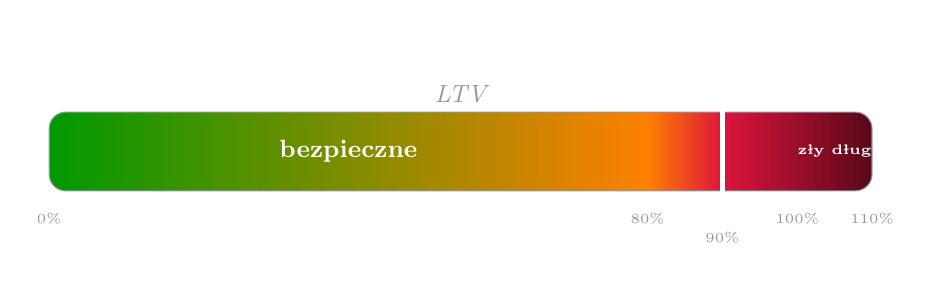
\begin{tikzpicture}[x=0.95cm,
        lbl/.style={font=\tiny\itshape, text=stplmuted},
      ]
      \begin{scope}
        \clip[rounded corners=6pt] (0,0) rectangle (11,1);
        \shade[left color=green!60!black,   right color=orange]           (0,0)  rectangle  (8,1);
        \shade[left color=orange,           right color=stplred]          (8,0)  rectangle  (9,1);
        \shade[left color=stplred,          right color=stplred!70!black] (9,0)  rectangle (10,1);
        \shade[left color=stplred!70!black, right color=stplred!40!black] (10,0) rectangle (11,1);
      \end{scope}
      \draw[rounded corners=6pt, draw=stplmuted, line width=0.4pt] (0,0) rectangle (11,1);
      \draw[draw=stplwhite, line width=1.5pt] (9,-0.5) -- (9,1.55);
      \node[font=\small\bfseries, text=stplwhite, above] at (9,1.55) {likwidacja};
      \node[lbl] at (0,-0.35)  {$0\%$};
      \node[lbl] at (8,-0.35)  {$80\%$};
      \node[lbl] at (9,-0.6)   {$90\%$};
      \node[lbl] at (10,-0.35) {$100\%$};
      \node[lbl] at (11,-0.35) {$110\%$};
      \node[font=\small\itshape, text=stplmuted, above] at (5.5,1) {LTV};
      \node[font=\small\bfseries, text=stplwhite] at (4,0.5)    {bezpieczne};
      \node[font=\tiny\bfseries,  text=stplwhite] at (10.5,0.5) {zły dług};
    \end{tikzpicture}
  \end{center}
  \vspace{0.15cm}
  \begin{itemize}
    \item \textbf{Loan-to-Value (LTV)} --- stosunek wartości pożyczki do wartości collateral
    \item \textbf{Health Factor (HF)} --- miara oddalenia pozycji od likwidacji; $HF < 1$ uruchamia likwidację
  \end{itemize}
\end{frame}

\begin{frame}{Utilization Rate}
  \begin{itemize}
    \item Niskie $U$ $\Rightarrow$ niskie APR (zachęta do pożyczania)
    \item Wysokie $U$ $\Rightarrow$ wysokie APR (zachęta do dostarczania płynności)
    \item \textbf{Kink model} --- gwałtowny wzrost oprocentowania po przekroczeniu progu optymalnego (np.\ $U = 80\%$)
  \end{itemize}
  \vspace{0.3cm}
  \begin{block}{\textbf{Utilization Rate}}
    \[
      U = \frac{\text{borrowed}}{\text{supplied}}
    \]
    Wskaźnik wykorzystania puli --- steruje oprocentowaniem.
  \end{block}
\end{frame}

\begin{frame}<1>{Utilization Rate --- wykres}
  \begin{center}
    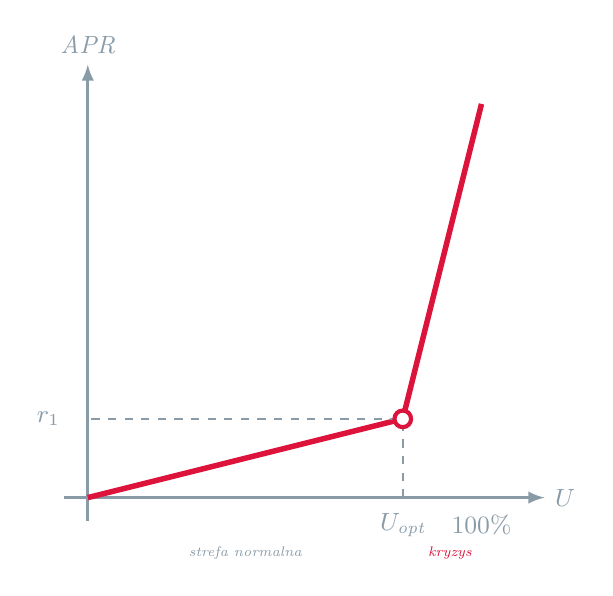
\begin{tikzpicture}[
        lbl/.style={font=\small\itshape, text=stplmuted},
      ]
      \draw[draw=stplmuted, -latex, line width=1pt]
        (-0.3,0) -- (5.8,0) node[right, lbl] {$U$};
      \draw[draw=stplmuted, -latex, line width=1pt]
        (0,-0.3) -- (0,5.5) node[above, lbl] {APR};

      % Kink model: gentle slope 0 → U_opt, steep slope U_opt → 100%
      \draw[draw=stplred, line width=2pt] (0,0) -- (4,1) -- (5,5);

      % Dashed reference lines at kink point
      \draw[draw=stplmuted, dashed, line width=0.6pt] (4,0) -- (4,1) -- (0,1);

      % Axis tick labels
      \node[lbl] at (4,-0.35) {$U_{\text{opt}}$};
      \node[lbl] at (5,-0.35) {$100\%$};
      \node[lbl] at (-0.5,1) {$r_1$};

      % Zone labels
      \node[font=\tiny\itshape, text=stplmuted] at (2,-0.7) {strefa normalna};
      \node[font=\tiny\itshape, text=stplred] at (4.6,-0.7) {kryzys};

      % Kink point
      \filldraw[fill=stplwhite, draw=stplred, line width=1.5pt] (4,1) circle (3pt);
    \end{tikzpicture}
  \end{center}
\end{frame}

% ================================================================
\section{Podsumowanie}

\begin{frame}{Podsumowanie}
  \begin{itemize}
    \item \textbf{Overcollateralized borrowing} --- zastaw broni protokół zamiast scoringu kredytowego
    \item Gdy wartość zastawu spada za nisko --- \textbf{likwidacja} automatycznie zamyka dług
    \item \textbf{Composability}: AMM i lending łączą się jak klocki --- leverage loop, yield aggregatory
    \item Trzecia lekcja --- programy i konta na Solanie
  \end{itemize}
\end{frame}

% ================================================================
\begin{frame}[plain]
  \begin{center}
    \vfill
    {\Huge\bfseries\color{stplwhite} gn}
    \vfill
  \end{center}
\end{frame}

\end{document}
